%*******10********20********30********40********50********60********70********80

\chap{Background Theory} 
\section{Data science}
It's really important to have a general idea about what "Data Science" means since this thesis procedure is strongly based on the classic Data Science Process.

We can define Data Science like a "concept to unify statistics, data analysis and their related methods" in order to understand and analyze actual phenomena with data.\\
It includes theories drawn from many field within the broad areas of mathematics, statistics, information science and computer science.

\begin{minipage}{0.5\textwidth}
In the computer science area are particular important the subdomains of:
\begin{itemize}
\item Machine learning
\item Classification
\item Cluster Analysis
\item Data mining
\item Databases
\item Visualization
\end{itemize}
\end{minipage} \hfill
\begin{minipage}{0.50\textwidth}
\begin{figure}[H]
	\centering
    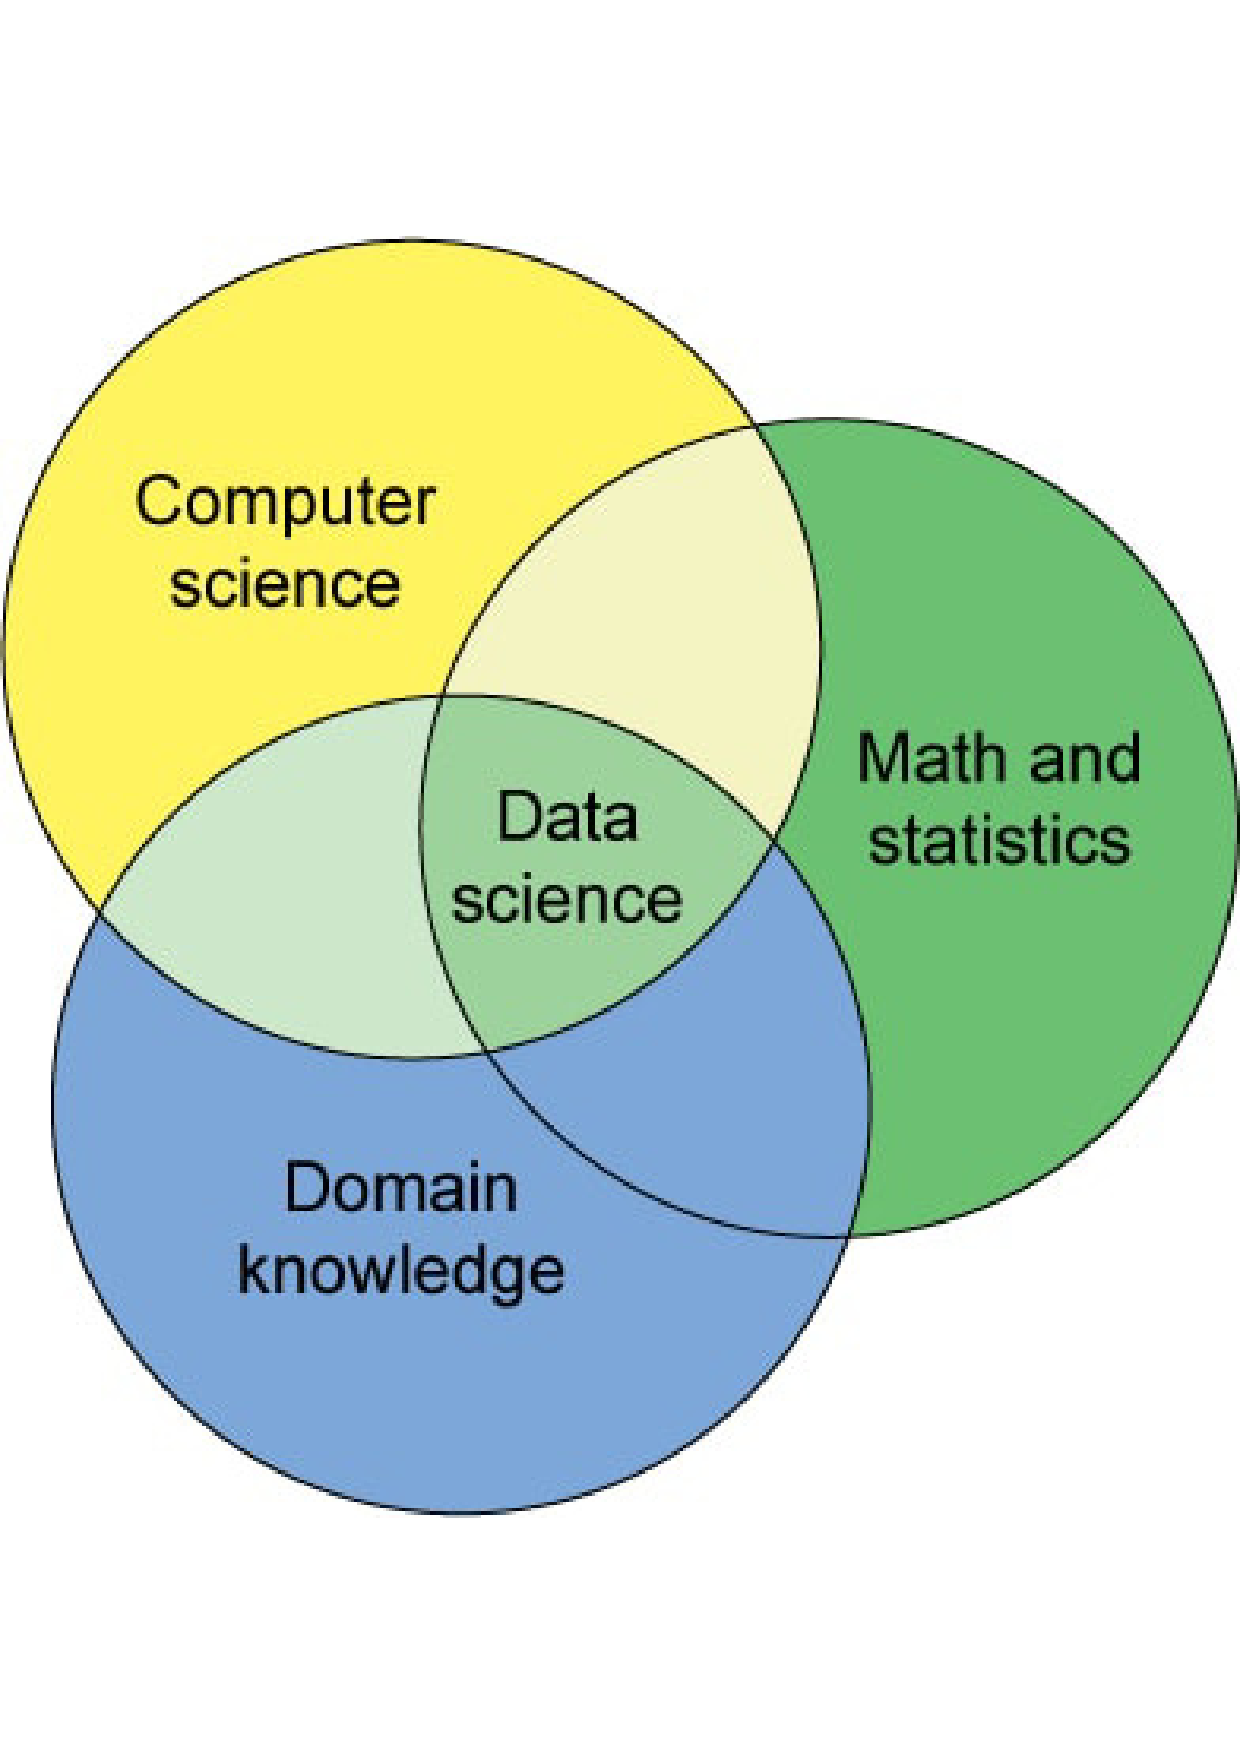
\includegraphics[trim={0 3cm 0 3cm},clip,width=0.9\textwidth]{Files/Data_Science_Concept.pdf}
    \caption{Data science concept}
    \label{fig: Data_science}
\end{figure}

\end{minipage}

\newpage 

Here is reported a short definitions about the main subdomains considered by this study:
\begin{itemize}

\item \textbf{Data mining}: Is the computing process of discovering patterns in large data sets. The overall goal of the data mining process is to extract information from a data set and transform it into an understandable structure for further use.

\item \textbf{Data Visualization}: It involves the creation and study of the visual representation of data. The primary goal of data visualization is to communication information clearly and efficiently via graphics and plots.

\item \textbf{Machine learning}: Is a subfield of computer science that, according to Arthur Samuel in 1959, gives computers the ability to learn without being explicitly programmed. More useful specific informations about this field are provided in the following section [\ref{ML}].
\end{itemize}

The follow image represents the "Blitzstein and Pfister's framework" and provides a clear overview of the Data Science process.
\begin{figure}[H]
    \centering
    \makebox[\textwidth][c]{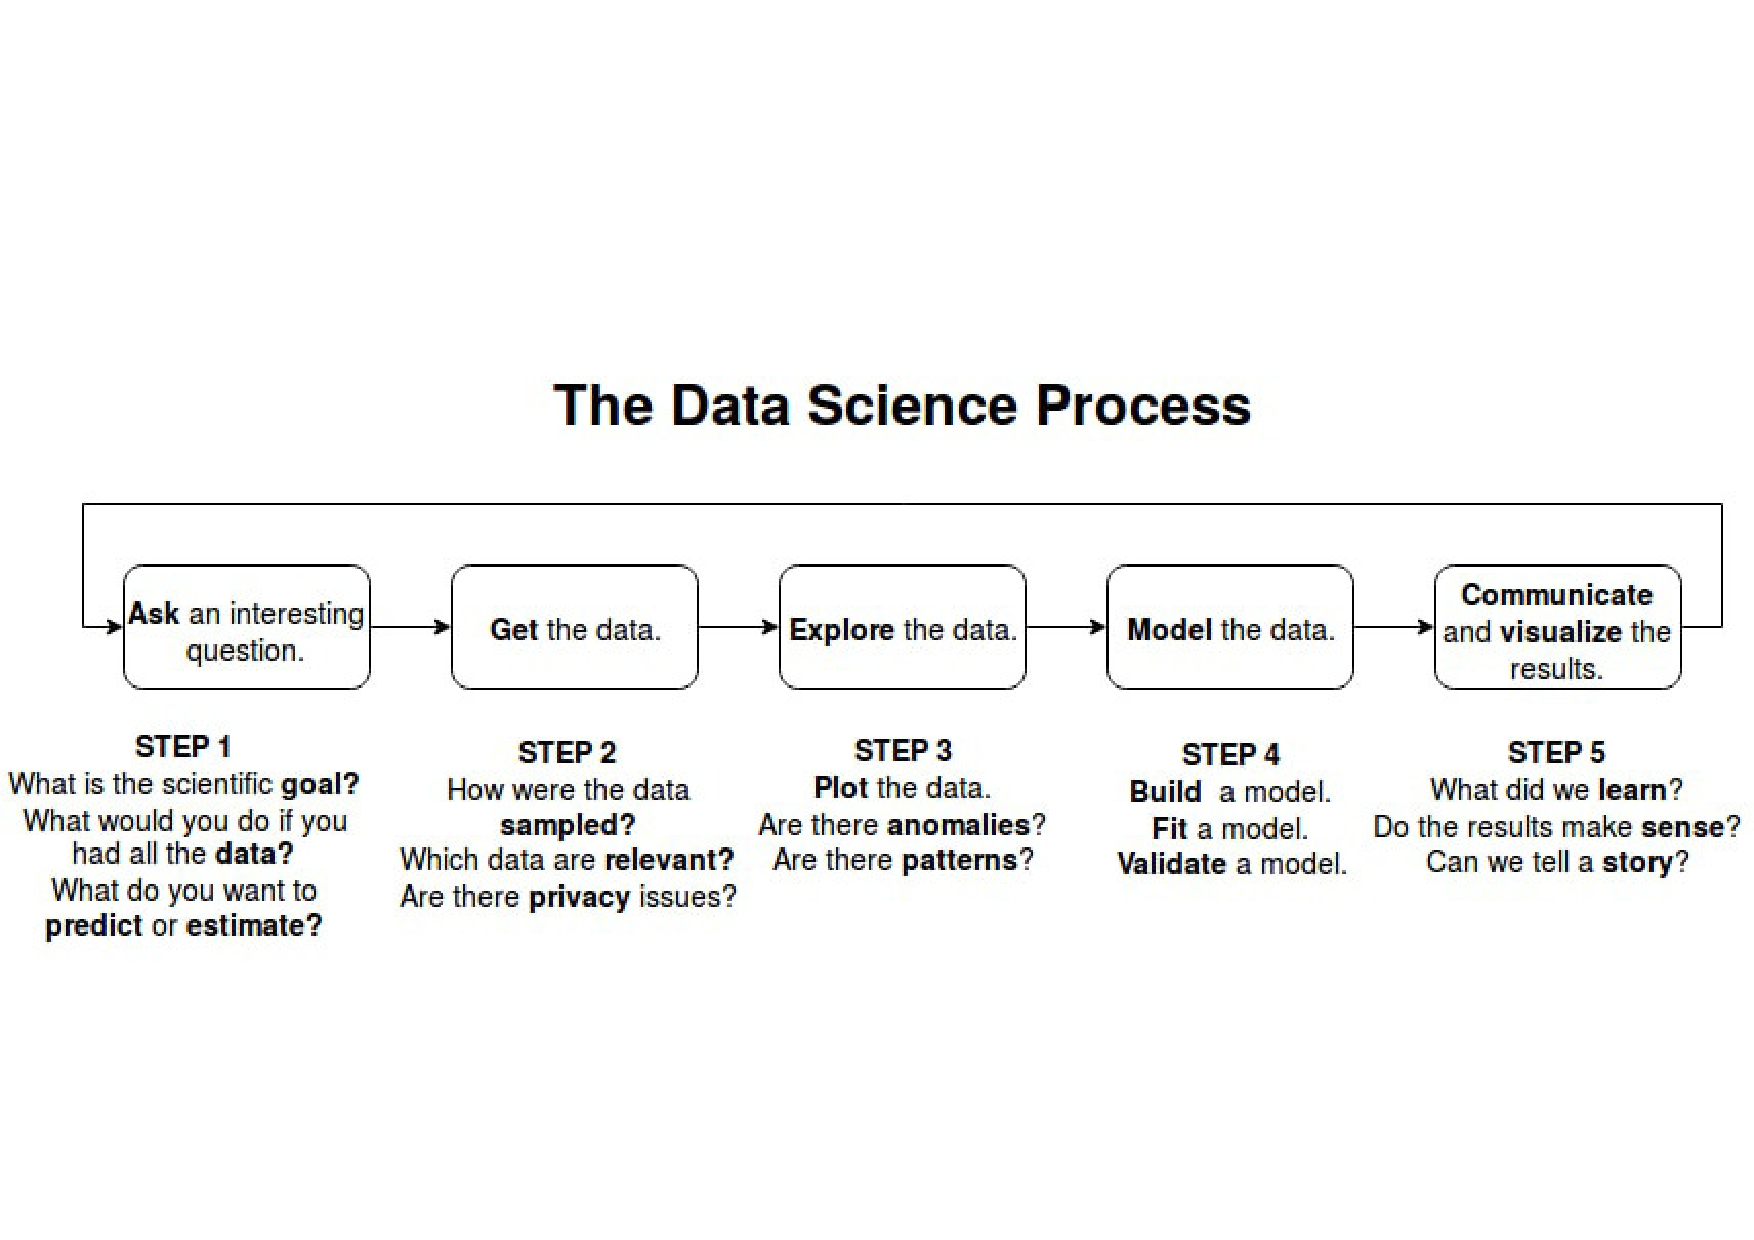
\includegraphics[trim={0 0 0 2cm},clip, width=1.2\textwidth]{Files/Data_Science_Process.pdf}}
    \caption[Data science process]{Data science process}
    \label{fig: Data_science}
\end{figure}



\newpage


\section{Machine learning}
\label{ML}
How is reported in the previous section, this subfield of computer science gives "computers the ability to learn without being explicitly programmed". \\
Machine learning explores the study and construction of algorithms that can learn from and make predictions on data.

There are several machine learning algorithm, each one of them is used for a different purpose and a different domain. For examples:
  \vspace{-5mm}
\begin{itemize}
 \setlength{\itemsep}{-5pt}
  \item Deep Learning
  \item Neural Network
  \item Regularization
  \item Clustering
  \item \textbf{Regression}: This specific domain contains the model used in this study.
  \item Bayesian
  
 \end{itemize}  

\subsection{Time Series analysis and predictions}
  \vspace{-5mm}
Time Series forecasting is an important area of machine learning, but that is often neglected. Is that important mainly beause there are so many prediction problems that involve a time component, and these problems are neglected because it is this time component that makes time series problems more difficult to handle.

" A time series is a sequence of observations taken sequentially in time. " \\
Quoted — Page 1, Time Series Analysis: Forecasting and Control.

Classic example of a time series dataset:

\begin{tabular}{ | l | l | }
\hline 		\textbf{Date}	&	\textbf{Paramater} \\ \hline
				Time \#1	&	observation \\ \hline	
				Time \#2	&	observation \\ \hline	
				Time \#3	&	observation \\ \hline											
\end{tabular}

Understanding a dataset is called time series analysis and it can helps to make better prediction, but sometimes it's not required and can result in a large of technocal investment in time and expertise.

Making predictions could be called time series forecasting and it involves taking models fit on historical data and using them to predict future observations.

\newpage 

\subsection{Autoregressive integrated moving average (ARIMA)}
\vspace{-5mm}
Since this a very complicated and deep topic, this study provided just an initial implementation and descripton of it.
During this section are provided some basic definitions and overviews enough to understand the general logic behind a forecasting system. If you are particular interested in this topic my suggestion is to read more about it, in the specific the mathematic side.\\

\textbf{AR model}: an autoregressive model is a representation of a type of random process; as such, it is used to describe certain time-varying processes in nature, economics, etc. The autoregressive model specifies that the output variable depends linearly on its own previous values and on a stochastic term (an imperfectly predictable term); thus the model is in the form of a stochastic difference equation.

\textbf{MA model}: a moving-average model is a common approach for modeling univariate time series. The moving-average model specifies that the output variable depends linearly on the current and various past values of a stochastic (imperfectly predictable) term. 

\textbf{ARMA model}: an autoregressive-moving-average model provides a parsimonious description of a stationary stochastic process in terms of two polynomials, one for the autoregression and the second for the moving average. Basically it combines both AR and MA models into a unique representation.

\textbf{ARIMA model}: is a generalization of an autoregressive moving average (ARMA) model. Both of these models are fitted to time series data either to better understand the data or to predict future points in the series (forecasting).\\
This model is applied in some cases where data show evidence of non-stationarity, where an initial differencing step (corresponding to the "integrated" part of the model) can be applied one or more times to eliminate the non-stationarity.

\textbf{ARIMA(p, d, q)}
  \vspace{-5mm}
\begin{itemize}
 \setlength{\itemsep}{-5pt}
\item \textbf{p} is the number of autoregressive terms (How many preceding values are examinated for the current value’s forecast).

\item \textbf{d} is the number of nonseasonal differences needed for stationarity.

\item \textbf{q} is the number of lagged forecast errors in the prediction equation. 
\end{itemize}

\newpage

\section{Aquaculture in Norway}

Is the aquaculture business in Norway growing? 
  
Aquaculture, also known as aquafarming, is the farming of fish, crustaceans, molluscs, aquatic plants, algae, and other aquatic organisms.

Aquaculture would be the future of fish:
In 2030, according to the World Bank, aquaculture will supply:
\begin{itemize}
\item 93.6 Million tonnes of fish per year
\item 25 percent less wild fish will be available
\item 62 percent of the fish we eat will come from farms
\end{itemize}




